\documentclass[12pt]{book}


\usepackage{exercises}
\RequirePackage{lineno}
\usepackage{graphicx}
%\usepackage{amsmath}
\usepackage[a4paper, total={6.3in, 8.5in}]{geometry}
\usepackage[super]{natbib}


%\usepackage{siunitx}
%\usepackage[version=3]{mhchem}
%\renewcommand*{\thefootnote}{\fnsymbol{footnote}}
%\graphicspath{ {../Figures/} }
\linespread{1}

\usepackage{geometry}
 \geometry{
 a4paper,
 left=20mm,
 right=20mm,
 top=25mm,
 bottom=20mm,
 }

% Makes nice font:
\renewcommand{\familydefault}{\sfdefault}

\newcommand{\DocTitle}{Climate Dynamics Course Notes}

\usepackage{fancyhdr}
\pagestyle{fancy}
\fancyhf{}
\rhead{Mauritsen}
\chead{}
\lhead{\DocTitle}
%\cfoot{Page \thepage}
\cfoot{}

% Remove to get numbers:
%\bibliographystyle{plainnat}
%\bibpunct{(}{)}{;}{a}{}{,}


\newcommand{\beginsupplement}{%
        \setcounter{table}{0}
        \renewcommand{\thetable}{S\arabic{table}}%
        \setcounter{figure}{0}
        \renewcommand{\thefigure}{S\arabic{figure}}%
     }

%
%\begin{document}
%
%
%\begin{center}
%\noindent
%{\LARGE 
%\DocTitle
%} \\
%\vspace{0.5 cm}
%
%\noindent
%{\bf Thorsten  Mauritsen$^{1*}$}\\
%\today \\
%\end{center}
%
%\noindent
%$^1$ Max Planck Institute for Meteorology, Hamburg, Germany \\
%%$^2$ University of Colorado, Boulder, USA \\
%%$^3$ NOAA Earth System Research Lab, Physical Sciences Division, Boulder, USA \\
%\\
%$^*$ Corresponding author: Thorsten Mauritsen, Max Planck Institute for Meteorology, Bundesstrasse 53, 20146 Hamburg, Germany, e-mail: thorsten.mauritsen@mpimet.mpg.de\\
%
%%\linenumbersK
%%\linenumbers
%%\modulolinenumbers[2]


\title{\DocTitle}
\author{Thorsten Mauritsen}
\date{\today}
 
\begin{document}
 
\maketitle
\tableofcontents

\frontmatter
\chapter{Preface}
Let us take a look at a planet from space -- and -- imagine we let time pass relatively quickly. From this perspective we can observe a system in approximate stationarity; something which we usually call equilibrium. This is not to be mistaken for a strict thermodynamical equilibrium, wherein, as you may have learnt in other courses, the system is characterised by a single well-defined temperature, but rather an approximate equilibrium between radiative energy received from the star around which our planet of interest is circulating (provided it does have a star), and the thermal energy that the planet is radiating to space. How does the planet come into equilibrium, and is there only one equilibrium? How does the equilibrium change if the star changes it's irradiance, or the planets orbit is altered? How does the equilibrium of the planet depend on properties of the planet? To begin to answer these questions we will have to dig into the processes that determine the energy balance, but the starting point will be our somewhat abstract perspective from space and time.

Usually we think of the climate as something that is static, we think of averages in time -- traditionally taken to be 30 years. So why discuss the dynamics of something that is static? The climate is varying on timescales as short as we choose to define them up to those of the existence of the planet (Figure \ref{fig:Paleo_temperature_timeseries}). These variations were either due to external factors, such as the sun, or  the composition of the atmosphere changing due to biogeochemical processes, or internal variability. Much of this can be described by simple dynamical equations, as the dynamics of climate. A related and interesting field describes the dynamics of the atmosphere- and ocean circulations and the biogeochemical cycles. 

\vspace{1.0 cm}
\noindent
{\bf \LARGE Scope of the course}
\\
\\
\noindent In the Climate Dynamics course I hope to bring you close to the forefront of current knowledge in climate dynamics, and ideally to inspire you to ask interesting questions on your own. Beyond this ideal, I hope to provide you with a solid basis for appreciating the stability of Earth's climate, and how and why we think it has, and is, changing. You will learn about forcing, feedback mechanisms and climate sensitivity, about the timescales involved in the climate system, and I will have a special focus on instrumental record warming. 

The course is theoretical in the sense that we will be working with abstraction: simple models that explain some aspect of the system in a distilled way, either ignoring a number of factors or condensing them into simpler formulations. We will work both analytically and with simple computational models. 


\begin{figure}
\begin{center}
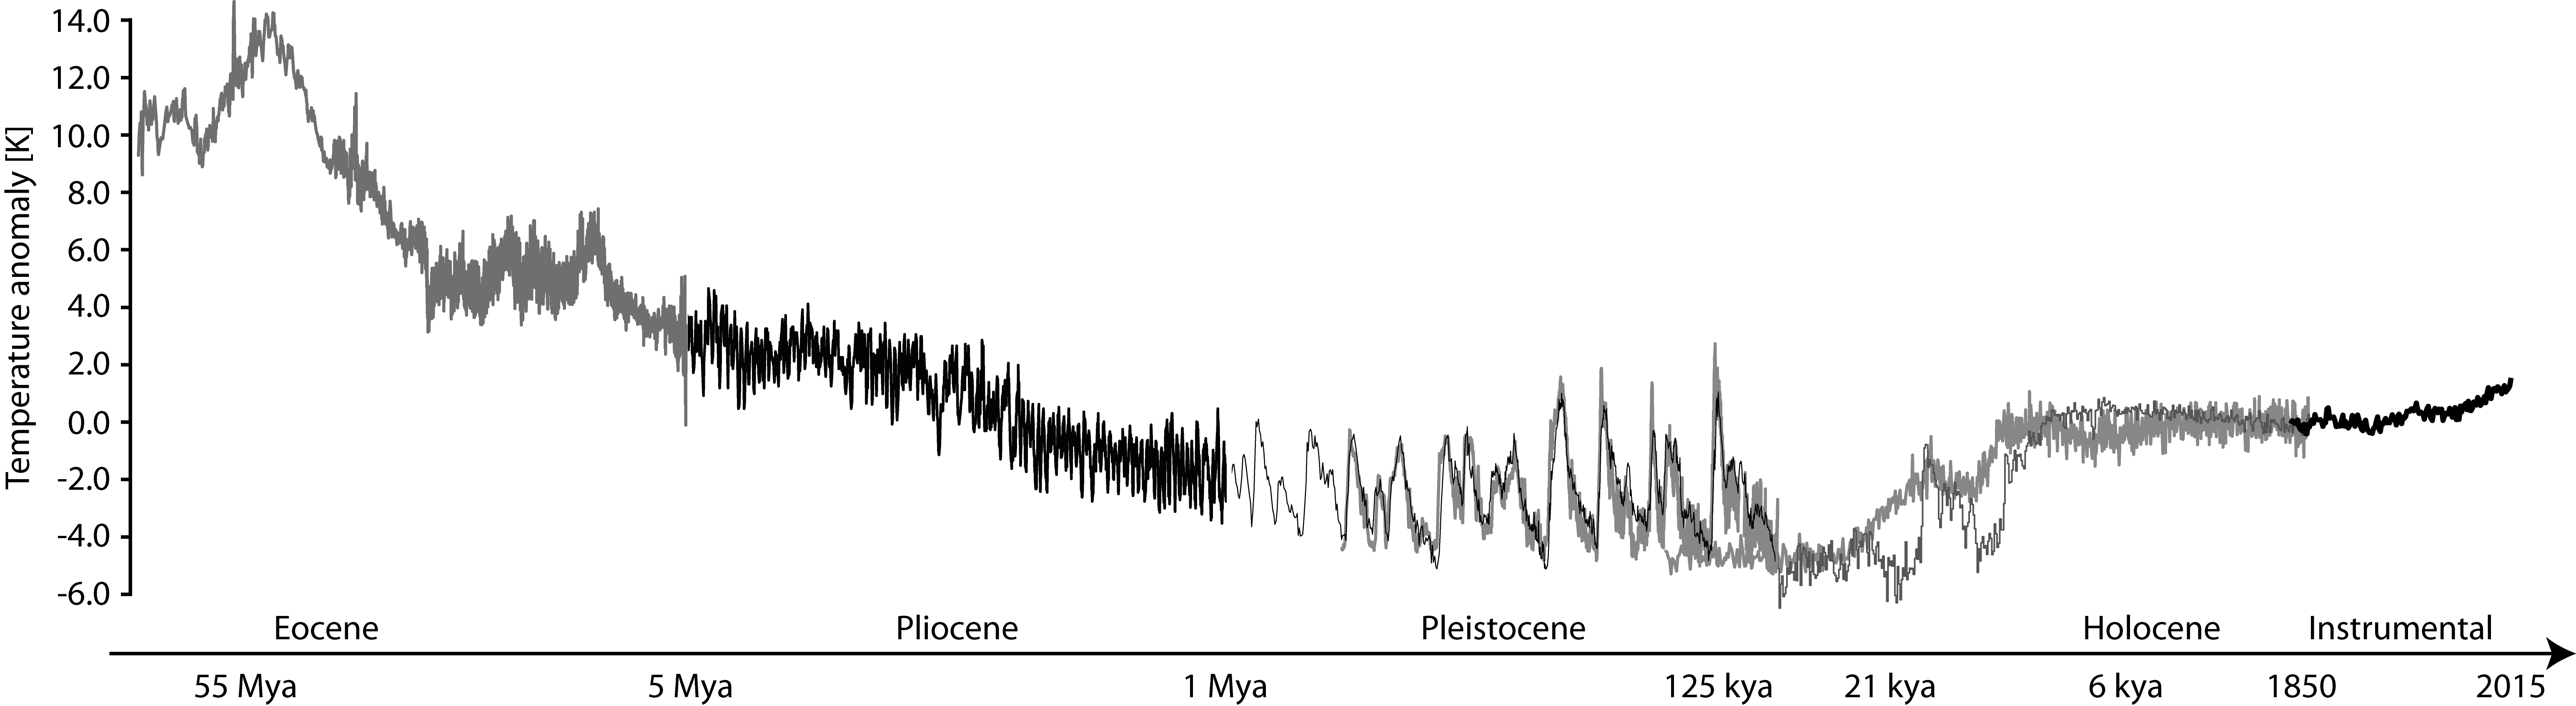
\includegraphics[width=17 cm]{../external_figures/Paleo_temperature_timeseries}
\end{center}
\caption{ Concatenation of various proxies of temperature from the past for illustration purposes. Note the logarithmic time-axis. Modified from the original by Glen Fergus. } 
\label{fig:Paleo_temperature_timeseries}
\end{figure}

\mainmatter
%---------------------------------------------------------------------
%---------------------------------------------------------------------
\chapter{Essentials}
\label{chapter:essentials}
Here I go over some of the basics of Earth's climatology, it's radiative properties and the energetic flows. This chapter is intended to provide a minimal background for the further studies. We will spend a bit extra time trying to understand what controls the height of the troposphere. 

\section{Temperature of the Earth and its atmosphere}
From basic thermodynamics we have learned that an isolated system has a well-defined temperature when it is in a thermodynamic equilibrium wherein there are only random brownian transfer of energy and no net fluxes exist. The Earth is very far from thermodynamic equilibrium, and instead about 173 Petawatt (PW: $10^{15}$W) are received from the sun and approximately the same amount is radiated to back to space in the form of reflected sunlight and as infrared radiation. In this case it makes sense to choose a more practical definition of Earth's temperature, for instance that which is needed temperature needed to achieve equilibrium: the warmer it is the more infrared radiation it will radiate to space. This is sometimes referred to as the Earth's radiation temperature at thermal equilibrium.

\begin{figure}
\begin{center}
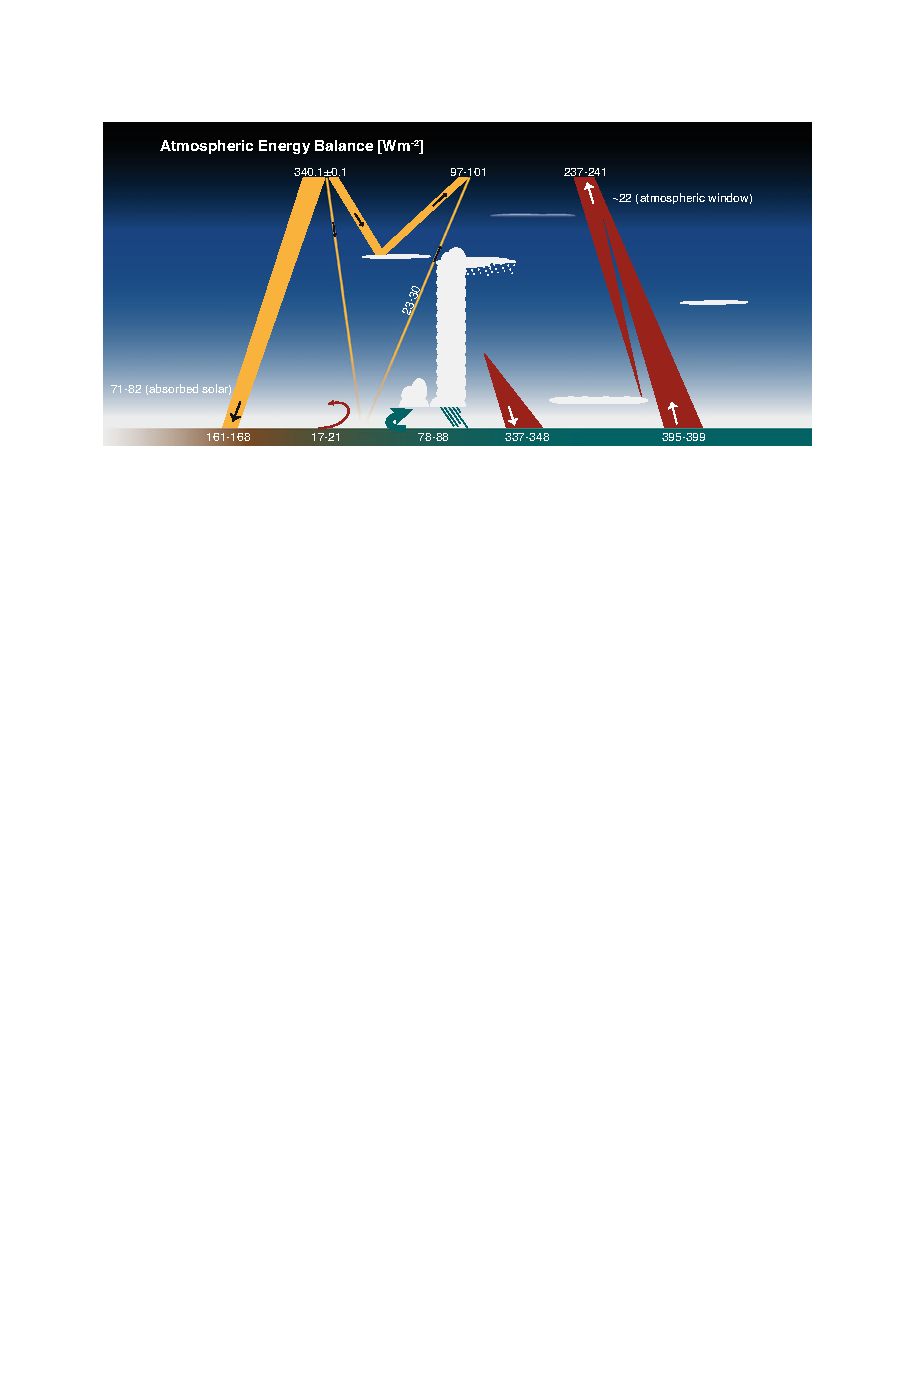
\includegraphics[width=15 cm]{../external_figures/Stevens_Schwartz_2012_energy_flows.pdf}
\end{center}
\caption{ Observational estimates of the Earth's energy balance from Stevens and Schwartz \citep{Stevens2012}. Yellow is sunlight, red is infrared radiation. The little whirl is turbulent sensible heat transfer and the green is latent heat transfer. } 
\label{fig:energy_flows}
\end{figure}

It is useful to consider the components of the global mean energy balance (Figure \ref{fig:energy_flows}). Here we consider the fluxes per meter squared surface area of the Earth (total area $510\cdot 10^{12}$ m$^2$). Energy flows in from the sun at 340 Wm$^{-2}$, about 100 of which are reflected back to space by clouds, aerosol particles or the surface. In the atmosphere some of the sunlight is absorbed, mostly by oxygen, ozone and water vapor, and the rest reaches and heats the surface. The surface gets rid of the heat again through emitting infrared radiation, and sensible and latent heat fluxes to the atmosphere. Of the emitted nearly 400 Wm$^{-2}$ infrared radiation most it is absorbed by the atmosphere

\begin{figure}
\begin{center}
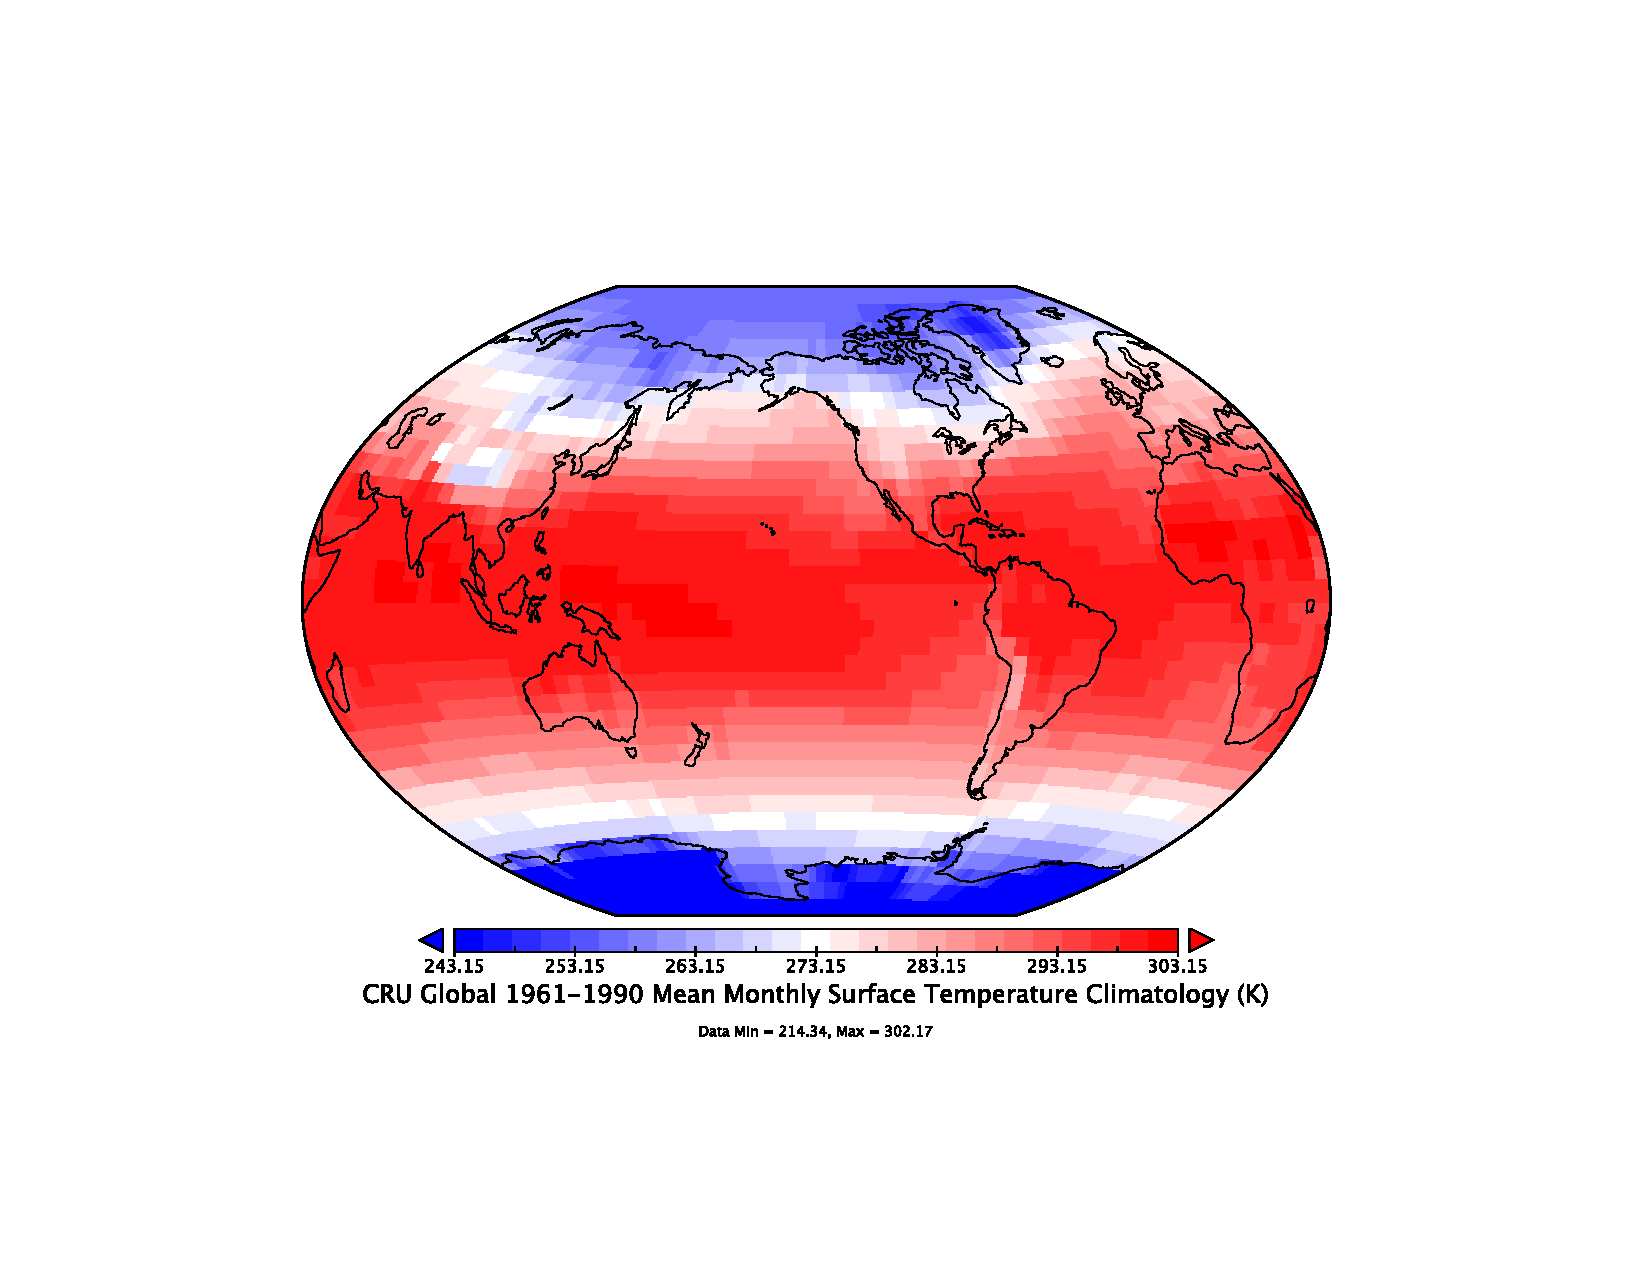
\includegraphics[width=12 cm]{../external_figures/HadCRUT_absolute_timmean.pdf}
\end{center}
\caption{ Observed annual mean near-surface temperature from HadCRUT. } 
\label{fig:HadCRUT_temperature_map}
\end{figure}

Partly because the sunlight is not distributed evenly over the Earth's surface it exhibits wildly varying temperatures near the surface with extremes from about -90$^\circ$C to +60$^\circ$C. Even in the annual longterm mean the coldest and warmest places differ by nearly 90 degrees (Figure \ref{fig:HadCRUT_temperature_map}). As we will see below, these temperature gradients set up large energy flows in the atmosphere and oceans from warmer to colder regions. Nevertheless, we will often use a global mean surface temperature; today this is about 15$^\circ$C.

On average, though, the coldest point in the Earth's troposphere is the tropical tropopause region with temperatures around 200 K (Figure \ref{fig:tropical_profiles}). These low temperatures are achieved through vertical mixing in deep convective clouds wherein localized rapidly rising motion causes adiabatic cooling due to the decreasing pressure with height. If the air was dry the temperature would decrease at a rate of about -10 K km$^{-1}$, but because some latent heat is released as water vapor condenses during the ascent, the actual lapse rate is less, about -6 K km$^{-1}$ as can be inferred from Figure \ref{fig:tropical_profiles}. This is referred to as the moist adiabat.

Unlike the horizontal temperature gradients at the Earth's surface, mostly from equator to poles, that cause energy to be transported in the oceans and the atmosphere, the vertical temperature gradient of about 100 K in the topical troposphere is not on it's own causing transports to occur. However, as we shall see in a moment radiative cooling causes an upward convective  transport of energy to balance the budget of the atmosphere.

\begin{figure}
\begin{center}
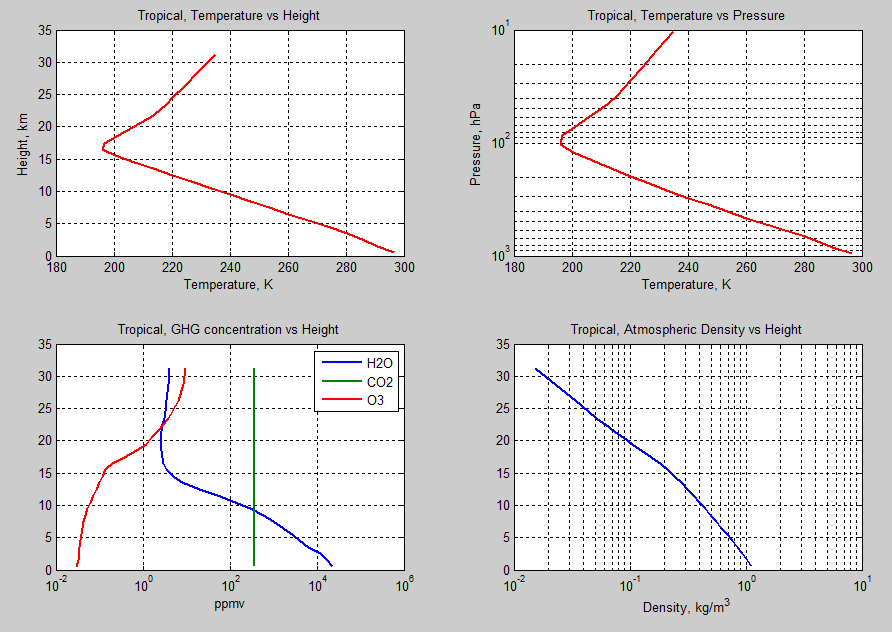
\includegraphics[width=17 cm]{../external_figures/atmospheric-radiation-13a-tropical-profile-temperature-gases-density}
\end{center}
\caption{ Typical profiles of temperature, greenhouse gases and density in the tropics.  } 
\label{fig:tropical_profiles}
\end{figure}

\section{Radiative properties}




Spectra

\begin{figure}
\begin{center}
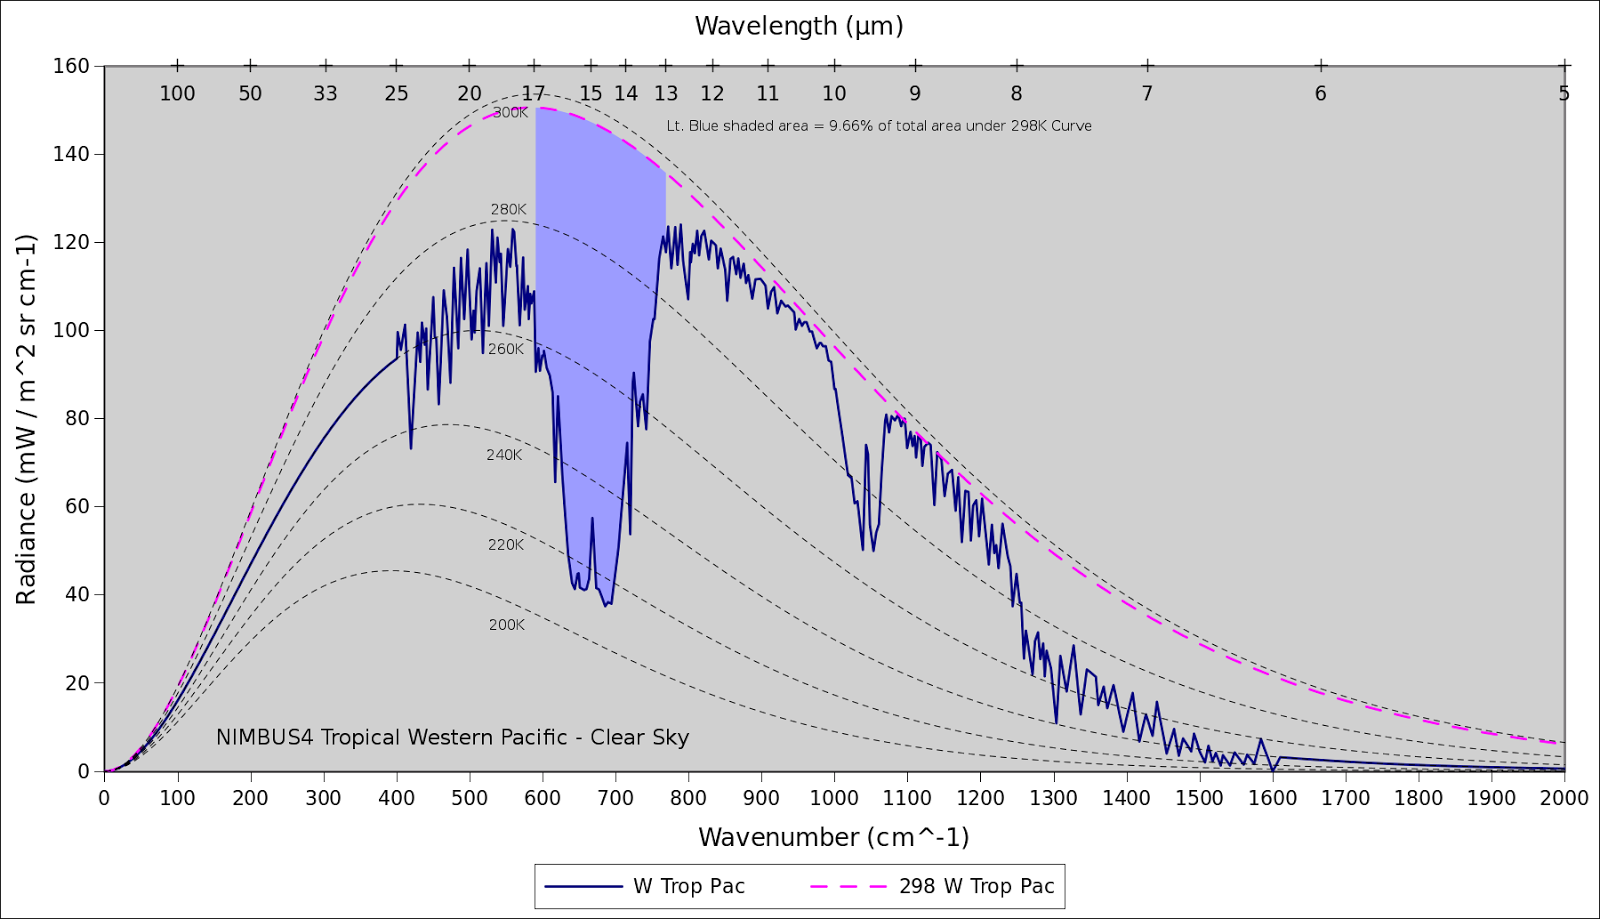
\includegraphics[width=17 cm]{../external_figures/GW_Petty_IRIS_Tropical_Western_Pacific.png}
\end{center}
\caption{ Classical irradiance spectrum measured by the infrared interferometer spectrometer (IRIS) for measuring the emission spectra of the earth/atmosphere system aboard the Nimbus-4 satellite. The instrument is limited to the range 400 to 1600 cm$^{-1}$, and outside simplistic extrapolations are made. The measurements were made in the 1970's and are restricted to clear sky scenes. Dashed lines show idealized black body spectra. Blue shading illustrates the effect of carbon dioxide (CO$_2$). The other dip at 1000-1100 cm$^{-1}$ is due to ozone (O$_3$), and the flanks (less than 600 and more than 1200 cm$^{-1}$) are dominated by vapor vapor (H$_2$O). } 
\label{fig:radiation_spectrum}
\end{figure}

Cooling rates (Petty 2006)

\begin{figure}
\begin{center}
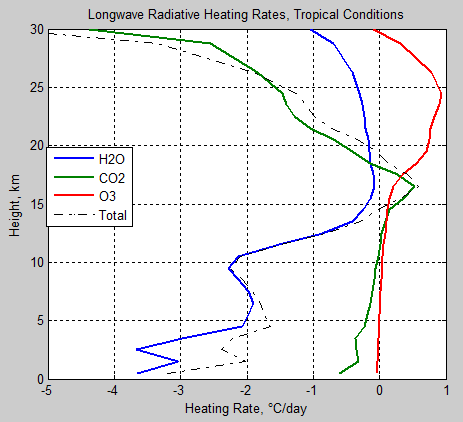
\includegraphics[width=8 cm]{../external_figures/atmospheric-radiation-13c-heating-rates-tropical-each-h2o-co2-o3.png}
\end{center}
\caption{ Longwave heating rates due to individual greenhouse gases calculated for the  clear-sky tropical atmosphere displayed in Figure \ref{fig:tropical_profiles}.  } 
\label{fig:radiative_cooling}
\end{figure}

\begin{figure}
\begin{center}
\includegraphics[width=12 cm]{../plots/CERES_Ebaf_zonalmean.pdf}
%\includegraphics[width=8 cm]{../plots/CERES_Ebaf_albedo.pdf}
\end{center}
\caption{ Top-of-atmosphere net fluxes of shortwave and longwave radiation as measured from satellite. The red area shows regions where more energy is received than emitted, it extends approximately from 36S to 36N and has a mean of 36.5 Wm$^{-2}$. The blue areas are regions that emit more radiation to space than they receive. In the Southern Hemisphere the mean flux is -54.0 Wm$^{-2}$ and in the Northern Hemisphere the deficit is -54.7 Wm$^{-2}$.  } 
\label{fig:ceres_fluxes}
\end{figure}


\section{The tropopause}

Radiative-convective equilibrium, ozone layer heating, tropopause

%\section{Energy transports}
%The atmosphere and oceans transport energy

\newpage
\vspace{1 cm}
\hrule
{\setlength{\parindent}{0cm}
\begin{exercise}
Estimate roughly from which heights in the troposphere thermal radiation to space comes from? Use Figures \ref{fig:tropical_profiles} and \ref{fig:radiation_spectrum} and divide into lower-, mid- and upper troposphere by means of its temperature. Use the fact that the area under the curve in Figure  \ref{fig:radiation_spectrum} is the total flux. Compare the amount of radiation escaping to space at near-surface brightness temperature to the amount escaping through the atmospheric window in Figure \ref{fig:energy_flows}. What is missing? From approximately which height do you think radiation in the wavelength range 9-10 $\mu$m come? 
\end{exercise}

\begin{exercise}
Explain, in your own words, why the tropopause is where it is.
\end{exercise}
}

% TASKS:
%
% Make sure you have python access, including numpy and matplotlib (preferably Anaconda)
%
% Assume the Earth's surface is a black body and calculate it's temperature based on the emission in Figure \ref{fig:energy_flows}. Assume it is 1 K warmer, then how much more does it radiate? How much of this flux will approximately escape directly to space through the atmospheric window?
%
% Estimate from which heights in the troposphere thermal radiation to space comes from
% Estimate the fixed anvil temperature (FAT) cloud feedback by assuming a fixed areal coverage of anvils and a fixed tropospheric lapse-rate
%
% Show that the short term response to an abrupt forcing does not depend on lambda.
%
% Show that T(t) is a solution to the two-layer model to an abruptly applied forcing, draw the two components of the solution as a function of time and their sum 
% 
% Assume a polynomial behavior of lambda, estimate max and minimum ECS
% Estimate steric sea-level rise in two-layer model
% Assume X percent of the top-of-atmosphere energy imbalance goes to 
%
% Does FAT depend on the temperature of the surface?

% Imagine one alternative cause of historical warming (e.g. solar forcing, ozone depletion, geothermal heating, galactic particles). How would you go about testing this hypothesis?

%---------------------------------------------------------------------
\chapter{Energy balance}
Let us take a look at the planet Earth from space. By focusing on 

\section{Stationarity}


\begin{equation}
N = \frac{S_o}{4}(1-\alpha) - \epsilon \sigma T_s^4,
\end{equation}
\noindent which for $N=0$ can be solved:
\begin{equation}
T_s = \sqrt[4]{S_o(1-\alpha)/4\sigma}
\end{equation}



\section{The greenhouse effect}

\section{A note on signs}
Throughout this set of notes I will count all fluxes as positive downwards. 

\vspace{1 cm}
{\setlength{\parindent}{0cm}
\hrule
\begin{exercise}
text
\end{exercise}
}

%---------------------------------------------------------------------
\chapter{Forcing, feedback and stability to small perturbations}

\section{Surface albedo feedback}
\section{Water vapor feedback}
\section{Cloud feedbacks}
\section{Radiative kernels?}

%---------------------------------------------------------------------
\chapter{Temporal evolution}
\section{Heat capacities and time-scales}
\section{Mixed-layer ocean}
%\subsection{Step-response solution}
\section{Two-layer model}
\section{Zero-layer model}
\section{Sea-level rise}

%---------------------------------------------------------------------
\chapter{Historical warming}

%---------------------------------------------------------------------
\chapter{Forcing and adjustments}

%---------------------------------------------------------------------
\chapter{Time- and state-dependent feedback}
\section{Snow-ball Earth instability}
\section{Runaway greenhouse}
\section{Ocean heat uptake efficacy}

%---------------------------------------------------------------------
\chapter{The water cycle}


%---------------------------------------------------------------------
%\chapter{The thermohaline circulation}






%\begin{figure}
%\begin{center}
%\includegraphics[width=8 cm]{../Commitment_estimates_plots/Figure_1_ECS_TCR}
%\end{center}
%\caption{ \small Probabilities of the transient climate response TCR and the equilibrium climate sensitivity ECS based on observed warming, estimates of historical radiative forcing and observations of present-day energy imbalance (a). The lower panel (b) shows the ratio of these quantities, which is roughly equivalent to the proportion of long-term warming realized on centennial time scales. Displayed numbers are the median and 5-95 percentiles of each distribution. } 
%\label{fig:ecs_tcr}
%\end{figure}

%--------------------------------------------------------%
\newpage
\bibliographystyle{naturemag}
\bibliography{bibliography}
%--------------------------------------------------------%

\vspace{5 mm}
\noindent
{\bf Acknowledgements} 



\newpage

\begin{table}
  \caption{Input for the observations-based analysis. Changes are between the period 2005-2015 minus 1859-1882. Uncertainties are standard deviations of the assumed gaussian distributions. The lower part of the table specifies the individual contributions to the total forcing change, whereas the total aerosol forcing ($F_\textrm{aero}$) is relative to 1750. }
  \vspace{0.5 cm}
  \centering
  \begin{tabular}{lrlr}
    \hline
    Quantity & Value &  & Source\\
    \hline
    Temperature change ($\Delta T$)     & 0.77&$\pm$ 0.08 K                  & HadCRUT4\citep{Morice:2012dw} \\
    Total forcing change ($\Delta F$)      & 2.16&$\pm$ 0.59 Wm$^{-2}$   & IPCC\citep{IPCC:2013is} \\    
    Planetary imbalance, 2005-2015 ($Q$)            & 0.71&$\pm$ 0.06 Wm$^{-2}$   & Johnson et al.\citep{Johnson:2016do} \\
    Planetary imbalance, 1859-1882                      & 0.15&$\pm$ 0.075 Wm$^{-2}$ & Lewis and Curry\citep{Lewis:2014jt} \\    
    \hline
    Greenhouse gas forcing change   & 2.53&$\pm$ 0.18 Wm$^{-2}$   & IPCC\citep{IPCC:2013is} \\    
    Aerosol forcing change                  &-0.69&$\pm$ 0.55 Wm$^{-2}$   & IPCC\citep{IPCC:2013is} \\    
    Black carbon on snow change      & 0.02&$\pm$ 0.02 Wm$^{-2}$   & IPCC\citep{IPCC:2013is} \\     
    Stratospheric water vapor change& 0.06&$\pm$ 0.03 Wm$^{-2}$   & IPCC\citep{IPCC:2013is} \\        
    Land use change                          &-0.10&$\pm$ 0.06 Wm$^{-2}$   & IPCC\citep{IPCC:2013is} \\        
    Ozone change                              & 0.29&$\pm$ 0.12 Wm$^{-2}$   & IPCC\citep{IPCC:2013is} \\        
    Contrails                                        & 0.05& Wm$^{-2}$                     & IPCC\citep{IPCC:2013is} \\        
    Natural forcing change                  & -0.005 &  Wm$^{-2}$                & IPCC\citep{IPCC:2013is} \\         
    \hline
    Forcing for doubled CO$_2$ ($F_{2\times}$)           & 3.71&$\pm$ 0.26 Wm$^{-2}$   & \\        
    Total aerosol forcing, 2005-2015 ($F_\textrm{aero}$)  &-0.90&$\pm$ 0.55 Wm$^{-2}$   & \\      
    \hline
  \end{tabular}

  \label{table:input}
\end{table}

\begin{table}
  \caption{ Input for calculation of short-lived climate forcers associated with fossil fuel burning. Uncertainties are standard deviations calculated from the referenced 5-95 percentiles. }
  \vspace{0.5 cm}
  \centering
  \begin{tabular}{lrlr}
    \hline
    Quantity & Value &  & Source\\
    \hline
    Methane (CH$_4$)              & 0.970 &$\pm$ 0.10 Wm$^{-2}$                  & IPCC\citep{Myhre:2013ui} \\
    Nitrogen oxides (NO$_x$)     & -0.151 &$\pm$ 0.11 Wm$^{-2}$                  & IPCC\citep{Myhre:2013ui} \\
    Carbon monoxide (CO)       & 0.234 &$\pm$ 0.03 Wm$^{-2}$                  & IPCC\citep{Myhre:2013ui} \\
    Fossil fuel fraction of CH$_4$ emissions ($f_{ff}$) & 0.29 &$\pm$ 0.02   & IPCC\citep{Ciais:2013ui} \\
    \hline
    Weighted sum (F$_\textrm{slcf}$)      & 0.36   &$\pm$ 0.12 Wm$^{-2}$                  & \\
    \hline
  \end{tabular}

  \label{table:slcfs}
\end{table}



\end{document}

